%!TEX encoding = UTF-8 Unicode

%!TEX root = ../compendium2.tex

\Lab{\LabWeekFIVE}

\begin{Goals}
%!TEX encoding = UTF-8 Unicode

%!TEX root = ../compendium2.tex

\item Kunna skapa en klass utifrån en textuell beskrivning. % av dess medlemmar.
%\item Kunna skapa en klass utifrån ofärdig kod och dokumentationskommentarer.
%\item Kunna införa privata attribut med lämpliga namn som representerar instansers förändringsbara tillstånd.
\item Kunna förklara skillnaden mellan klasser och instanser av klasser.
\item Kunna förklara skillnader och likheter mellan ett singelobjekt och objekt som är instanser av klasser.
\item Kunna förklara skillnaden mellan förändringsbara och oföränderliga objekt.
%\item Förstå innebörden av instansreferensen \code{this}.
\item Kunna skapa och använda klasser vars instanser innehåller referenser till andra instanser (aggregering).

\end{Goals}

\begin{Preparations}
\item \DoExercise{\ExeWeekFIVE}{05}, speciellt uppgift \ref{exe:classes:labprep}.
\item Läs igenom hela laborationen och planera ditt arbete.
\end{Preparations}

\subsection{Bakgrund}

{\raggedright%
\begin{minipage}{0.56\textwidth}
\begin{figure}[H]
  \centering
  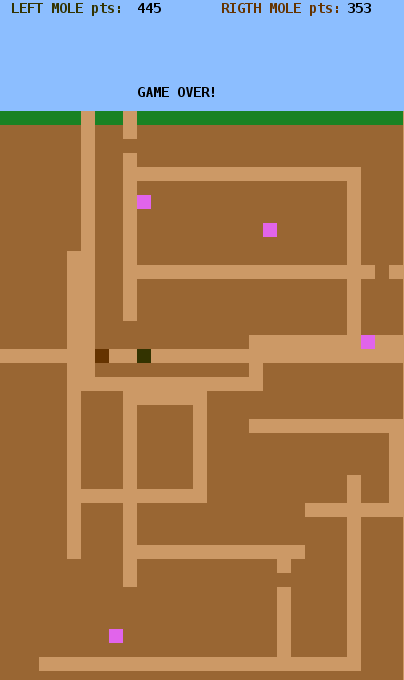
\includegraphics[width=\textwidth]{../img/blockbattle.png}
%  \caption{En lundensisk blockmullvad fångad på bild under aktivt grävanade.}
  \label{lab:blockbattle:fig:game}
\end{figure}
\end{minipage}%
}%
\newlength{\currentparskip}%
\newlength{\currentparindent}%
{
\setlength{\currentparskip}{\parskip}% save the value
\setlength{\currentparindent}{\parindent}% save the value
\hfill%
\begin{minipage}{0.4\textwidth}
\setlength{\parskip}{\currentparskip}% restore the value
\setlength{\parindent}{\currentparindent}% restore the value
\noindent Under denna laboration ska du träna på att deklarera klasser och skapa flera instanser av samma klass. Du tränar även på att bygga ett större program från grunden.

Du ska utveckla ett spel för två spelare som sitter vid samma tangentbord, där den vänstra spelaren styr en blockmullvad med tangenterna A,S,D,W, och den högra spelaren styr en annan blockmullvad med piltangenterna.

I bilden till höger ser du hur spelet kan se ut. Det finns en ljusbrun och en mörkbrun mullvad. Poängräkningen visas överst i himlen. Det finns fyra rosa blockmaskar (se uppgift \ref{lab:blockmole:task:blockworm} i laboration \code{blockmole}) som mullvadarna tävlar om att försöka fånga. När en blockmask teleporterar sig till en ny slumpmässig position lämnar den jord efter sig. När en mullvad är vid gräsytan lämnar den jord efter sig.
Det ger poäng att gräva tunnlar och att fånga blockmaskar.

Du bestämmer själv hur poängsättningen ska ske och kriteriet för när spelet är slut etc.
\end{minipage}%
}



\subsection{Obligatoriska krav}

Följande krav ska uppfyllas av din implementation:
\begin{itemize}[nosep, label={$\square$},]
%\item Det ska finnas två blockmullvadar, en för vänster spelare och en för höger spelare, som styrs med ASDW resp. piltangerna.
\item Varje mullvad rör sig i sin aktuella riktning tills användaren ändrar riktning genom att trycka på ''sin'' motsvarande knapp, t.ex. W eller pil-upp.
\item Då en mullvad går i mörkbrun jord grävs ljusbruna tunnlar.
\item Då en blockmullvad når fönstrets kant eller himlen ska mullvadens riktning bli den motsatta.
\item Det ska finnas poängräkning för varje spelares blockmullvad som visas under spelets gång.
\item Det ska ge poäng att gräva tunnlar.
\item Ett spel ska avslutas när något valfritt kriterium uppfyllts och texten \emph{Game over} ska då skrivas ut i spelfönstret.
\item Vid \emph{Game over} ska användaren kunna välja att avsluta programmet eller att starta ett nytt spel.
\end{itemize}

\vspace{1em}\noindent Din kod ska uppfylla dessa krav:
\begin{itemize}[nosep, label={$\square$}]
\item Du ska utgå från klasserna som du implementerat i uppgift \ref{exe:classes:labprep} i övning \texttt{\ExeWeekFIVE}.
\item Varje klass med ev. tillhörande kompanjonsobjekt ska finnas i en egen kodfil och tillhöra paketet \code{blockbattle}.
\item Det ska finnas en klass \code{Game} som skapas i huvudprogrammet och som har en metod \code{start()} som sätter igång spelet.
\item Konstanter ska, om lämpligt, namnges och placeras i kompanjonsobjekt.
\item Din kod ska kunna byggas med hjälp av byggverktyget \code{sbt}, se appendix \ref{appendix:build}.
\end{itemize}


\subsection{Valfria krav -- välj minst ett}

Välj själv att implementera minst ett, gärna fler, av följande krav:
\begin{itemize}[nosep, label={$\square$}]
\item Det ska finns ett lagom antal blockmaskar, förslagsvis 4 stycken i början.
\item Blockmullvadarna ska även ha ett heltalsvärde som representerar hälsan. Hälsan minskas något när man gräver tunnlar. Hälsan ska synas i spelfönstret.
\item Att springa på gräset ska ge poäng men kosta i hälsa.
\item Att fånga blockmask påverkar poäng och/eller hälsa.
\item Det ska finnas gula blockdiamanter som ger många poäng om man tar dem först.
\item Det ska gå att välja namn på sin blockmullvad och namnet ska synas i spelet vid poängutskriften.
\item Det ska gå fortare att gå i gångar jämfört med att gräva i jord.
\item Den blockmullvad som fångar en blockmask ska öka sin grävhastighet.
\item Vid varje \emph{Game Over} ska \emph{highscore} visas.
\end{itemize}

\subsection{Förebredelser inför redovisningen}
Innan du redovisar din implementation, förbered dig genom att vara beredd på att muntligt kunna redogöra för följande:
\begin{itemize}[nosep, label={$\square$}]
  \item Beskriv hur ditt program är organiserat.
  \item Beskriv vilka åtgärder du gjort för att koden ska vara lätt att läsa.
  \item Beskriv hur du stegvis utvecklat ditt program från enklare till mer avancerad funktionalitet, samt vilka buggar du upptäckt och fixat.
  \item Beskriv vilket eller vilka valfria krav som din implementation uppfyller.
  \item Beskriv hur du hade behövt ändra i klassen \code{Mole} för att det ska gå att skriva \code{new Mole.move().move().reverseDir().move()}
\end{itemize}

\subsection{Tips och goda råd}


% \begin{figure}[H]
% \scalainputlisting[numbers=left,basicstyle=\ttfamily\fontsize{9.8}{11.8}\selectfont]%
% {../workspace/w05_turtle/src/main/scala/graphics/RectSeq.scala}
% \label{code:classes:graphics:rectanglesequence}
% \end{figure}


%\Task En riktig utmaning, för den som har lust: Implementera spelet ''Masken'' som beskrivs här: \url{https://sv.wikipedia.org/wiki/Snake}.
